% Section 2 The Model Specification starting on page 605
\documentclass{article}
% List all of the packages used in all of the files, which can the just be added as an input.
\usepackage[margin=1in]{geometry}
\usepackage{titlesec}
\usepackage{amsmath}
\usepackage{subfiles}
\usepackage{mathptmx}
\usepackage{csvsimple-l3}
\usepackage[T1]{fontenc}
\usepackage[utf8]{inputenc}
\usepackage{tabularx,ragged2e,booktabs,caption}
\usepackage{tikz}
\usepackage[colorlinks=true,allcolors=blue]{hyperref}
\usepackage{graphicx}
\usepackage{changepage}
\usepackage{natbib}
\usepackage{longtable}
\usepackage{abstract}
\usepackage{atbegshi}% http://ctan.org/pkg/atbegshi
%% LaTeX path to the root directory of the current project, from the directory in which this file resides
% and path to econtexPaths which defines the rest of the paths like \FigDir
\providecommand{\econtexRoot}{}\renewcommand{\econtexRoot}{..}
\providecommand{\econtexPaths}{}\renewcommand{\econtexPaths}{\econtexRoot/TeXtools/econtexPaths}
% Mimicing professor's "ugly" solution to enable sharing base code between local LaTeX compilation and Overleaf

\providecommand{\FigDir}{\econtexRoot/FigDir}
\providecommand{\DataDir}{\econtexRoot/Data}
\providecommand{\SectionDir}{\econtexRoot/Sections}
\providecommand{\AppDir}{\econtexRoot/Appendices}
\providecommand{\TablesDir}{\econtexRoot/Tables}


\begin{document}

\section{THE MODEL SPECIFICATION}
\label{section:model}
In this section, we present a life-cycle model for an individual agent who rationally chooses his optimal life-cycle path for consumption and hours of labor supply. \par
At a given calendar time period $s$ and age $t$, the agent's period utility of consumption is a concave function of the consumption of market goods, $C$, and the disutility of labor is a convex function of the hours of labor supply $h$ and the taste shock $\epsilon_2$. Preferences are additively separable over time. Agents choose optimal consumption and labor supply by maximizing their discounted expected life-cycle
utility over the working horizon $T$, which is

\begin{equation} \tag{1}
\label{eq:LCU}
% Eq. 1 from paper, discounted expected life cycle utility
E_t \sum_{\tau=t}^T \beta^{\tau} [u(C_{\tau} , \tau) - v(h_{\tau} \epsilon_{2,\tau})]
\end{equation}

Agents also face an intertemporal budget constraint and a human capital production constraint. \par
The intertemporal budget constraint is
\begin{equation} \tag{2}
  \label{eq:IBC}
% Eq. 2 from paper the IBC
A_{t+1} = (1 + r)A_t + W_{t,s}h_t - C_t
\end{equation}

where $A_t$ is the agent's asset holdings at age $t$ and $r$ is the interest rate. The observed wage $W_{t,s}$ at age $t$, time $s$ is defined as the product of the human capital stock $K_t$ times the rental rate on a unit of human capital, $R_s$
\begin{equation} \tag{3}
W_{t,s}=R_sK_t
\end{equation}

The rental rate $R_s$ is the market price of services of a unit of human capital. We assume a perfect market for human capital. Hence, at any time $s$, all agents face the same rental rate $R_s$. \par
Human capital evolves according to the human capital production function, which is a deterministic function of current labor supply hours $h_t$, current human capital $K_t$, and age $t$, along with the multiplicative wage shock, $\epsilon_t$. That is,
\begin{equation} \tag{4}
  \label{eq:HCevolution}
  K_{t+1} = g(h_t, K_t, t) \epsilon_{1,t+1}
\end{equation}
$K_{t+1}$ is the age $t+1$ human capital after the wage shock $\epsilon_{1,t+1}$ is realized. \par
At age $t$, time period $s$, the agent's decision process can be described by the following maximiation of the value function.
\begin{equation} \tag{5}
  \begin{split}
      V_{t,s}(A_t,K_t,\epsilon_{2,t})=\text{max}_{C_t,h_t} & \{u(C_t,t)-v(h_t, \epsilon_{2,t}) \\ & + \beta E_t V_{t+1,s+1}[(1+r)A_t + R_s K_t h_t \\ & -C_t, g(h_t,K_t,t)\epsilon_{1,t+1}, \epsilon_{2,t+1}]\}
  \end{split}
\end{equation}
    For the utility function for consumption $C$, we choose a CRRA form augmented to include age effects
    \begin{equation*}
      u(C_t,t)=A(t)\dfrac{C_t^{a_1}}{a_1}
    \end{equation*}
    where $A(t)$ is a spline in age, and $a_1<1$ is a constant.\footnote[4]{The reason that age effects are needed to explain observed consumption behavior is as follows: In the data, wages and labor supply are both relatively small on average when people are young compared to when they are at prime age. Hence, annual labor income is low when people are young. Therefore, if people smooth consumption, they should be in debt when young, and repay it in later years of the life cycle. But this is not the case in the data. (See Table 3 for mean age profiles of wage, hours, and assets.) Thus, age effects in consumption are necessary to explain the positive asset holdings for youths observed in the data. To capture this, the utility of consumption should be smaller when young, so that consumption rises over time, and individuals would not go heavily into debt early in life. Alternative mechanisms to explain the observed asset pattern would be liquidity constraints, as in \cite{KeaneandWolpin2001}, or a more general utility function with a very strong precautionary saving motive. \par
The age effect $A(t)$ starts at $C_0 C_1$ at age 20, then gradually changes to $C_0 C_2$ at age 25 and to $C_0$ at age 33. Thereafter, $A(t)$ stays constant at the value $C_0$. That is, $A(t)$ is a linear spline with kinks at age 25 and 33. Agents in our model attempt to equate the marginal utility of consumption across time. If they place less value on consumption when young, this would be reflected in $C_1 < 1$ and $C1 + C2 < 1$. Then, at younger ages, less consumption is necessary to reduce the marginal utility of consumption to a given level.} \par
The disutility of labor, which is a function of hours $h$, is assumed to have the following functional form:
\begin{equation} \tag{6}
  v(h_t, \epsilon_{2,t} =  \epsilon_{2,t} b \dfrac{h_t^{a_2}}{a_2}
\end{equation}
where $b > 0$ and $a_2 > 1$ are constants. Except for the added age effects in the marginal utility of consumption, the functional forms are adopted from \cite{MaCurdy1981-iy} and \cite{Altonji1986-zf}.\footnote[5]{ By introducing intratemporal nonseparability of consumption and labor supply, one could explain the consumption profiles in the data without resorting to the age effects in consumption. But that would make the results of the estimation and simulation exercises less comparable to the results by \cite{MaCurdy1981-iy} and \cite{Altonji1986-zf}.} That will enable us to compare our results and theirs in later estimation and simulation exercises. Furthermore, in this parameter specification, the degree of intertemporal substitution of labor supply can be summarized by a single parameter, which is
\begin{equation*}
  i.e.s. \equiv b_2 \equiv \dfrac{1}{a_2-1}
\end{equation*}
Many empirical articles analyzing intertemporal labor supply behavior, such as \cite{Shaw1989-jb} or \cite{Hotz1988-gl}, use a translog function of consumption and leisure as the utility function. Although this approach has the advantage of being locally flexible, none of the parameters can be straightforwardly interpreted as describing the intertemporal elasticity of substitution in labor supply. Hence, from their estimation results, it is difficult to draw any conclusions about how much people substitute labor intertemporally, unless one simulates their estimated models.\footnote[6]{ Furthermore, in contrast to our full solution method, they use an Euler equation GMM method of estimation. There are some shortcomings of GMM estimation that are particularly related to the estimation of an intertemporal labor supply model that explicitly incorporates human capital accumulation, such as \cite{Shaw1989-jb}. That is, potential nonconcavities in agents' problem as a result of human capital investment may create problems for GMM. If we think of labor supply as an input to income production, then an increase in labor supply by A percent in every period results in an increase in wage income of more than A percent. That is because an increase in labor supply also raises future wages via human capital accumulation. Hence, there are increasing returns to scale in the income-generating process and potential nonconvexities in the model. In such a case, just looking at the first-order conditions may not be sufficient to claim that agents are solving the intertemporal optimal labor supply problem. In our estimation process, we explicitly solve for the continuous variable dynamic programming problem and embed the solution in the ML estimation. Hence, our solution truly assumes that individuals choose optimal labor supply and consumption over the life cycle. Furthermore, the full solution method leads to straightforward simulation of the model after the estimation. The main goal of this research is to simulate the intertemporal labor supply model to conduct some estimation exercises to highlight the potential bias of the conventional estimation methods.} \par
We assume the human capital production function in Equation \eqref{eq:HCevolution} to be as follows:
\begin{equation} \tag{4a}
g(K,h,t) = k_0 + \delta K + G(K,h,t)
  \end{equation}
  where $G(\cdot)$ is a function of current human capital, labor hours, and age $t$. Figure~\ref{fig:HCprodfunc} gives some evidence on the shape of the human capital production function from the NLSY79 data. The figure shows the relationship between current labor supply hours and the next period hourly wage rate, within different cells for the current wage.
%\hypertarget{HCprodfunc}{}
\begin{figure}[tbp]
  \centerline{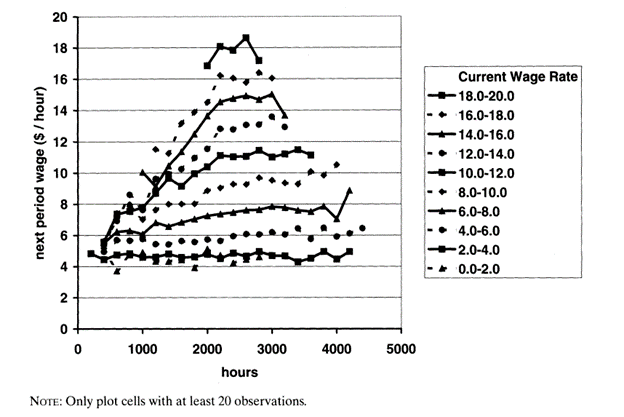
\includegraphics[width=6in]{../FigDir/Figure2.png}}
  \caption{HUMAN CAPITAL PRODUCTION FUNCTION} 
  \label{fig:HCprodfunc}
\end{figure}

\hypertarget{HCprodfunc}{}
\begin{figure}[tbp]
  \centerline{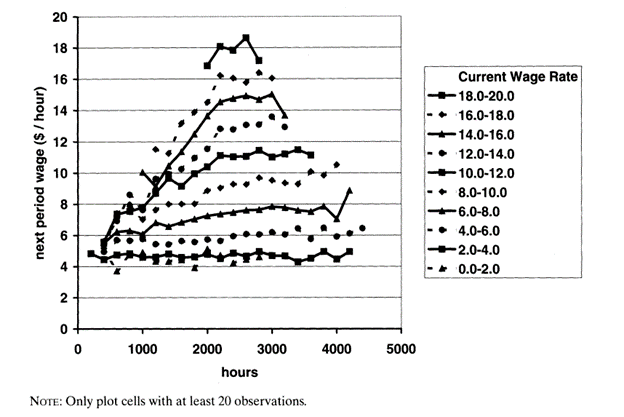
\includegraphics[width=6in]{../FigDir/Figure2.png}}
  \caption{HUMAN CAPITAL PRODUCTION FUNCTION} 
  \label{fig:HCprodfunc}
\end{figure}

  Each cell has length 2 dollars. In light of this evidence, the $G(\cdot)$ component of the human capital production function is specified as follows:
  \begin{equation} \tag{4b}
    G(K,h,t) = A_0(1 + A_1(t-19))(B_1+K)[(h+d_1)^{\alpha} - B_2(h+d_1)]
  \end{equation}
  This is designed to take account of the following features of the relationship between current hours, current wage rate, and the next period wage rate:
  \begin{enumerate}
  \item . The relation of future wages to current labor hours has a higher slope when the current wage is higher. That implies there is a significant complementarity between current wages and current hours in terms of learning by doing, which is captured by the multiplicative term $(B_1 + K)$.
  \item The derivative of the human capital production function with respect to hours around $h = 0$ appears to be bounded. We capture that by introducing the intercept term $d_1$.
  \item For very large hours, the slopes of the relation between future wages and current hours seems to be close to zero or even negative. Thus, there is a possibility that for very large hours, increase in hours have no effect on future human capital or even decrease future human capital. We can account for this possibility by adding the term $-B_2(h+d_1)$.
  \end{enumerate}
For estimation, we also include a pure age effect in the human capital production function, similar to the age effect included in the human capital earnings function by \cite{Keane1997-mg}, which corresponds to the term $A_1(t - 19)$. The wage and taste shocks are assumed to have i.i.d. mean one log normal distributions. That is,
  \begin{equation} \tag{7}
    \text{ln} (\epsilon_i) \sim N(-\frac{1}{2} \sigma_i^2, \sigma_i),~~~i=1,2
  \end{equation}
We also allow for the measurement errors in wages, labor supply hours, and assets. We defer the discussion of the measurement error functional forms until Section \ref{section:MLE}. \par
We set the working horizon $T$ at age 65. At the terminal period, we assume that agents get positive values from holding assets. This would arise, for example, because they are able to enjoy consumption until their death, and possibly can leave bequests to their heirs. We choose the following parameterization for the terminal value function:
\begin{equation} \tag{8}
  V_{T+1}(A_{T+1}) = \begin{cases}
        3 \log(A_{T+1} + \phi) - 1 - 3 \log(\phi) & \mbox{ if $A_{T+1}>0$}\\
        (\frac{A_{T+1}-\phi}{\phi})^3 & \mbox{ otherwise}
            \end{cases}
          \end{equation}
          where $\phi$ is a parameter that determines the marginal value of assets (at $T + 1$) at various asset levels. Higher values of 0 imply that agents care less about the terminal assets. We chose this specification because this function is continuously differentiable in assets and the derivative is decreasing in assets. \footnote[7]{The function is continuous at $A_{t+1}=0$ since
            \begin{equation*}
              \text{lim}_{A_{T+1} \downarrow 0} V_{T+1} (A_{T+1}) = 3 \log(0 + \phi) - 1 - 3 \log \phi = -1
            \end{equation*}
            and
            \begin{equation*}
              \text{lim}_{A_{T+1} \uparrow 0} V_{T+1} (A_{T+1}) = (\dfrac{0-\phi}{\phi})^3 = -1
            \end{equation*}
            Furthermore, the function is continuously differentiable at $A_{T+1}=0$ since for $A_{T+1}>0$,
            \begin{equation*}
             \dfrac{\partial V_{T+1} (A_{T+1})}{\partial A_{T+1}}|_{A_{T+1}>0} = \dfrac{3}{A_{T+1}+\phi} \to \frac{3}{\phi}
           \end{equation*}
           as $A_{T+1} \searrow 0$ and
           \begin{equation*}
             \dfrac{\partial V_{T+1} (A_{T+1})}{\partial A_{T+1}}|_{A_{T+1} \leq 0} = 3 (\frac{1}{\phi})^3(A_{T+1}-\phi)^2 \to \frac{3}{\phi}
           \end{equation*}
           as $A_{T+1} \nearrow 0$. Since both
           \begin{equation*}
             \dfrac{\partial V_{T+1} (A_{T+1})}{\partial A_{T+1}}|_{A_{T+1}>0} = \dfrac{3}{A_{T+1}+\phi}
           \end{equation*}
           and
            \begin{equation*}
             \dfrac{\partial V_{T+1} (A_{T+1})}{\partial A_{T+1}}|_{A_{T+1} \leq 0} = 3 (\frac{1}{\phi})^3(A_{T+1}-\phi)^2|_{A_{T+1} \leq 0}
           \end{equation*}
           are decreasing in $A_{T+1}$, the derivative is decreasing in assets.
         } It turns out that the coefficient $\phi$ is difficult to estimate (i.e., the likelihood is very flat over a wide range of 0), because the NLSY79 only has data on individuals until the age 36. After some experimentation, we set 0 to be 100,000. \footnote[8]{Since we only have data until the age 36, and the final period is at age 65, our experimentation indicated that the likelihood function is very flat for a wide range of $\phi$ values around 100,000. But if $\phi$ is larger than 200,000, the lack of concavity of the final period value function causes the continuous variable DP solution algorithm to break down.} \par
         Now, to understand the effect of introducing human capital accumulation on the hours response to wage changes, we consider the first-order conditions of the above problem with respect to consumption and labor. These are:
         \begin{equation} \tag{9}
           \label{eq:FOC}
           \begin{split}
             C_t: &  u_C(C_t,t) - \beta E_t V_{A,t+1,s+1}(A_{t+1},K_{t+1},\epsilon_{2,t+1}) = 0 \\
             h_t: & -v_h(h_t,\epsilon_{2,t}) + R_sK_t u_C(C_t,t) \\
             & + \beta E_t g_h \epsilon_{1,t+1} V_{K,t+1,s+1}(A_{t+1},K_{t+1},\epsilon_{2,t+1})=0
           \end{split}
           \end{equation}
          
           Notice that the current marginal disutility of labor equals the wage ($R_s K_t$) times the marginal utility of consumption, which is the marginal return to increases in current wage income due to increases in labor supply, plus an extra term that captures the marginal return to increases in future human capital. As the wage increases over the life cycle, the substitution effect induces labor supply to increase, thus providing an incentive for people to supply more labor in older age. This corresponds to the term $R_s K_t u_C(C_t, t)$. On the other hand, both concavity of the value function with respect to human capital and the approaching retirement period lower the marginal rate of return to human capital investment, thus reducing the incentive to supply labor. This comes from the term $\beta E_t g_h \epsilon_{1,t+1} V_{K,t+1,s+1}(A_{t+1}, K_{t+1}, \epsilon_{2,t+1})$. If these two factors roughly cancel, then even if wages increase over the life cycle, labor supply will be little changed (see Figure~\ref{fig:OptimalSupply}).\par
           Observed heterogeneity is introduced into the model by allowing the parameters $b,~C_0,~C_1,~C_2$ in preferences, and $K_0,~\delta,~A_0,~A$, and $\alpha$ in the human capital production function, to differ depending on whether an agent is a high school dropout, high school graduate, has some college, or is a college graduate. Completed schooling is treated as exogenous. We do not allow for unobserved heterogeneity, but, as we discuss in Section \ref{section:estimation}.4, the model is nevertheless able to generate substantial persistence in wages, hours, and assets due to the persistent nature of shocks to the human capital production function. \par
           At this point, readers who are not interested in the algorithms for solving the dynamic programming problem and forming the likelihood can skip Sections \ref{section:solving} and \ref{section:MLE} and go directly to the data description in Section \ref{section:data}.          
\end{document}
